\chapter{Metodologia}

Este trabalho utiliza o índice S4, uma lista de estações que realizam medidas desta variável e o VTEC. O trabalho também a ideia de pesquisa reprodutível, com códigos documentados, para tal se faz uso da tecnologia de ``notebooks"~em Python. Além disso, os ``notebooks"~estão disponíveis em \url{https://github.com/retiarus/tese}, juntamente com um conjunto de dados para teste. 

Os dados de S4 foram originalmente disponibilizados em formato de texto, juntamente com uma lista de estações ao longo do território brasileiro. Cada arquivo contém uma lista de medidas ordenadas pelo tempo, com múltiplas medidas por minuto, cada uma associada a um satélite. A etapa inicial consistiu em armazenar e organizar estes dados em um banco de dados, pois então, técnicas como filtragem permitem uma rápida seleção inicial dos dados por estação e elevação. Também foi adicionado ao banco de dados uma tabela com informações sobre as estações.

Os notebooks estão organizados tal que os primeiros dois dígitos indiquem, estabeleçam, uma ordem de execução, por exemplo, o notebook com inicial $00$ precisa ser executado antes do notebook com inicial $01$. Existem notebooks com os mesmos valores de dígitos, isto significa que um não apresenta dependência em relação ao outro e podem ser executados ao mesmo tempo.

\section{Seleção inicial dos dados de S4 e estações}

Este notebook realiza uma consulta a tabela de estações no banco de dados. Utilizando, então, a lista de estações retornada faz iterativamente uma consulta para cada estação selecionando apenas medidas cuja elevação é superior a 30.0. Somente continuam as estações que contém dados, gerando assim, uma tabela com os dados das estações, que entender-se-á como o conjunto inicial de estações, e um grupo de arquivos com dados de S4, um para cada estação válida. Os dados de S4 armazenados em uma tabela ordenada, indexada pelo tempo, podem ser vistos como uma série temporal.

\section{Gerando a série espaço-temporal para os dados de VTEC}

Os dados de VTEC estão inicialmente organizados em arquivos de texto, as duas primeiras linhas são de cabeçalho, onde a primeira, denota o instante dos dados, e a segunda fornece o significado de cada coluna. A primeira coluna é a longitude, a segunda a latitude e a terceira o VTEC. Medidas de VTEC $999.000$ denotam ausência de valor. Finalmente, cada arquivo constitui um mapa de VTEC, onde cada linha fornece o valor de VTEC para um ponto no espaço. Assim, o papel do notebook 00\_generate\_vtec\_dataframe.ipynb é o de converter este conjunto de arquivos em um tabela, indexada pelo tempo, onde cada linha contém uma matriz, que realiza o papel do mapa. Pode-se observar esta estrutura também como uma série espaço-temporal, onde um índice de tempo indexa um mapa de VTEC. Este notebook também realiza um ordenamento temporal nos dados, o que é necessário posteriormente para o cálculo de derivadas temporais, traduzidas aqui como diferenças finitas no tempo.

\section{Gerando um mapa das estações com os meridianos magnéticos} 

O notebook 01\_show\_stations.ipynb realiza um ordenamento na tabela de estações por estado e cidade. Seguindo de um agrupamento por cidade, uma vez que existem cidades com mais de um estação, e neste trabalho se adotou empregar apenas uma estação por cidade. 

Por meio do pacote Python AACGMV2, que implementa um modelo numérico para o sistema de coordenadas geomagnética AACGM, foi possível gerar as latitudes e longitudes geomagnéticas para as estações, utilizando os dados de localização geográfica, altitude, bem como uma data de referência.

Utilizando os dados geomagnéticos se plotou um mapa contendo as estações, assim, como os meridianos magnéticos que passam por estas. Lembrando-se que as bolhas ionosféricas evoluem ao longo dos meridianos magnéticos, tem-se que este mapa fornece uma visualização das estações que tendem a apresentam maior correlação entre si, pois pertencem a uma mesma eventual trajetória.

\begin{figure}[H]
\centering
\makebox[\textwidth][c]{\includesvg[width=1.6\columnwidth]{./Figuras/map_stations.svg}}
\label{fig:mapstations}
\caption{Representação dos meridianos magnéticos que atravessam as estações que realizam medidas de cintilação ionosférica.}
\end{figure}

\section{Suavização da série temporal de S4}

O notebook 02\_preprocessing\_s4\_data.ipynb é utilizado para o pré-processamento dos dados de S4. Primeiramente, toma-se o valor médio de todas as medidas realizada por minuto, isto é, realiza-se uma reamostragem combinando as medidas de diferentes satélites feitas no mesmo minuto, tal que se tenha um valor de S4 por minuto. 

Após esta etapa é feita uma interpolação spline de ordem 4 para tratar instantes sem amostras. Em seguida, é feita uma reamostragem para intervalos de 10 min, novamente utilizando o valor médio como função de agregação. O intervalo adotado é o mesmo do dados de VTEC. Nas figuras \ref{fig:savgol} e \ref{fig:gaussian} é possível observar em azul uma amostra do sinal S4, pode-se notar que este apresenta rápidas flutuações e ruído. Assim, optou-se por aplicar uma função de suavização. Em \ref{fig:savgol}, tem-se a utilização do filtro de Savitzky–Golay com janela de 9 pontos e polinômio interpolador de terceira ordem, enquanto na figura \ref{fig:gaussian} foi utilizado um filtro baseado em média móvel com pesos gaussianos com uma janela também de 9 pontos.

\begin{figure}[H]
\centering
\makebox[\textwidth][c]{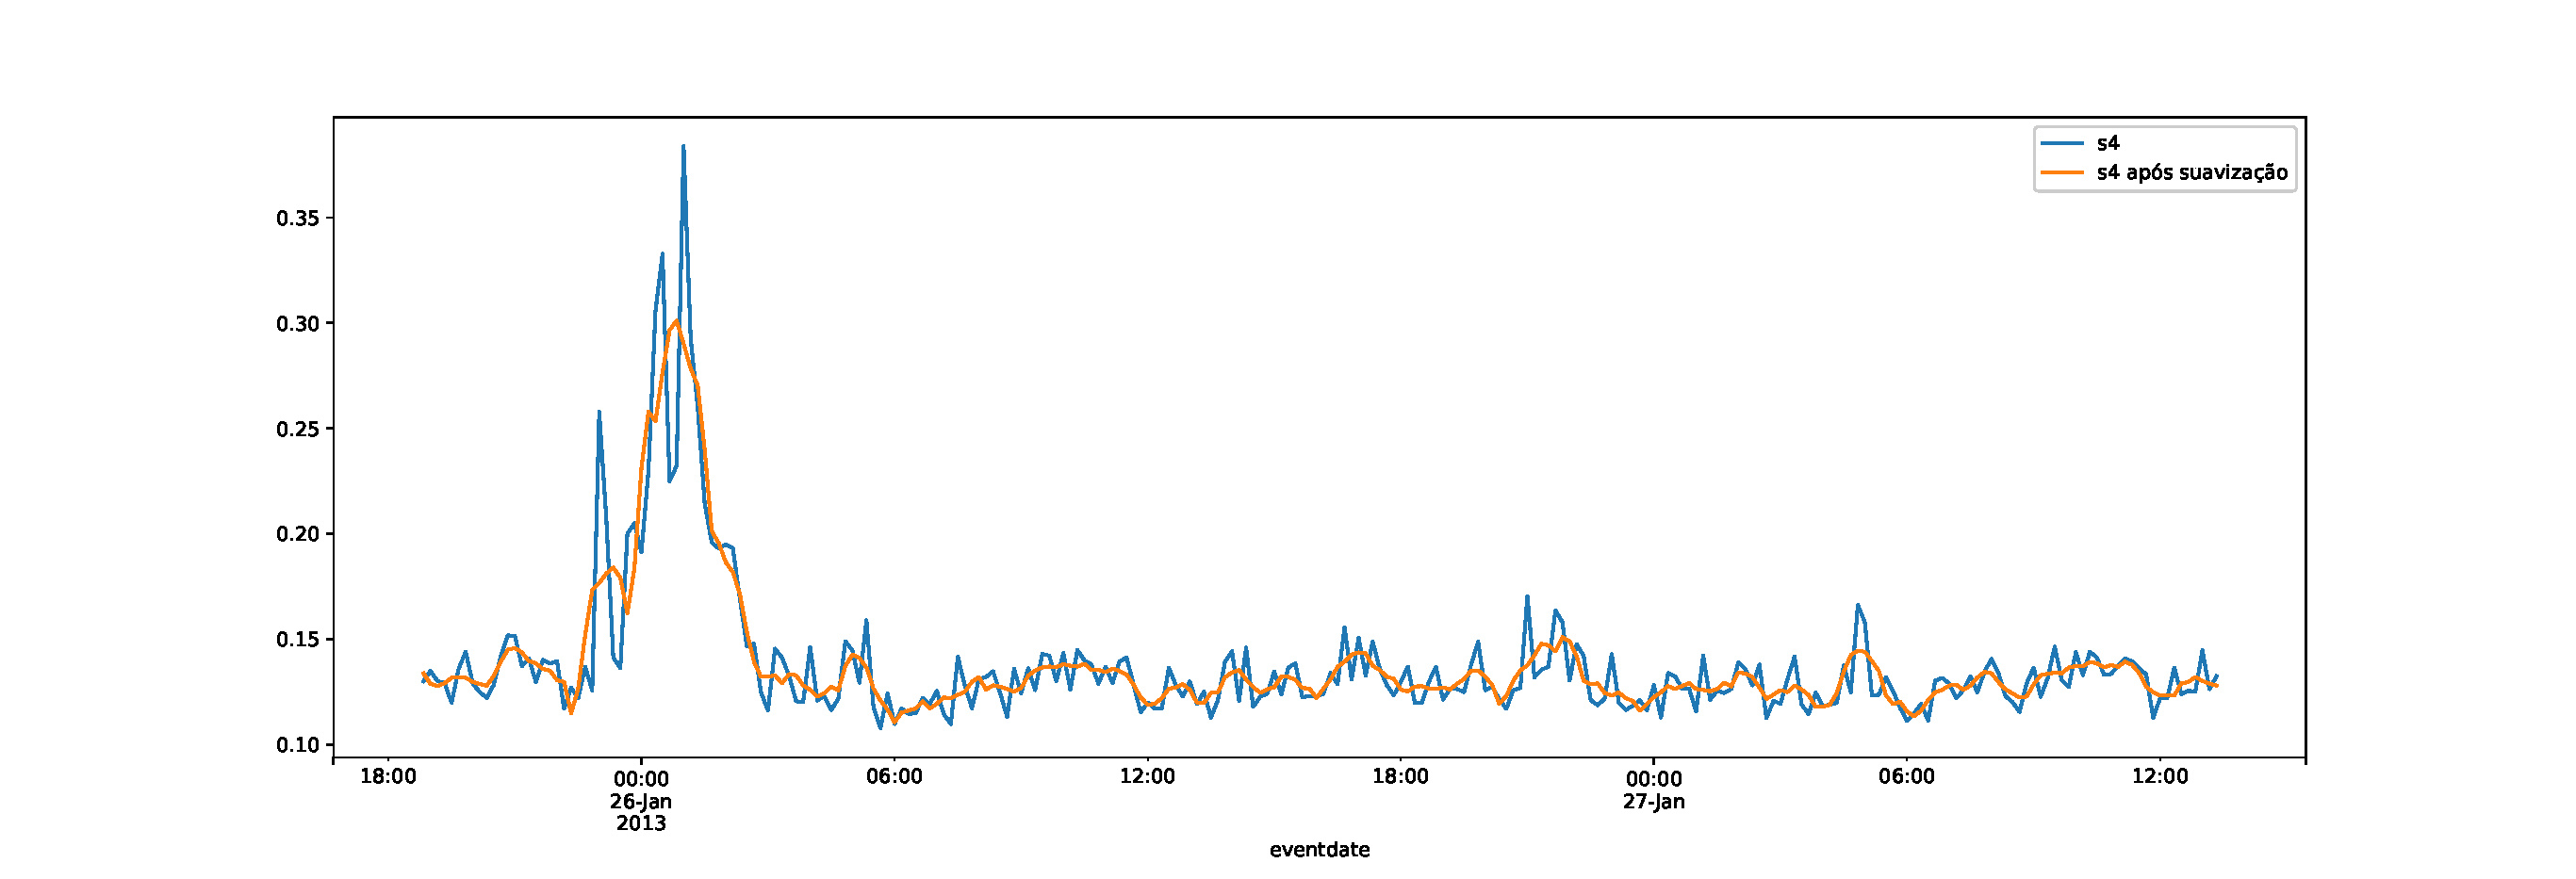
\includegraphics[width=1.4\linewidth]{./Figuras/s4_signal_noise_and_smooth_savgol.eps}}
\caption{Suavização de uma amostra da série temporal de S4, por meio do filtro de Savitzky–Golay.}
\label{fig:savgol}

%\vspace{-12pt}

\makebox[\textwidth][c]{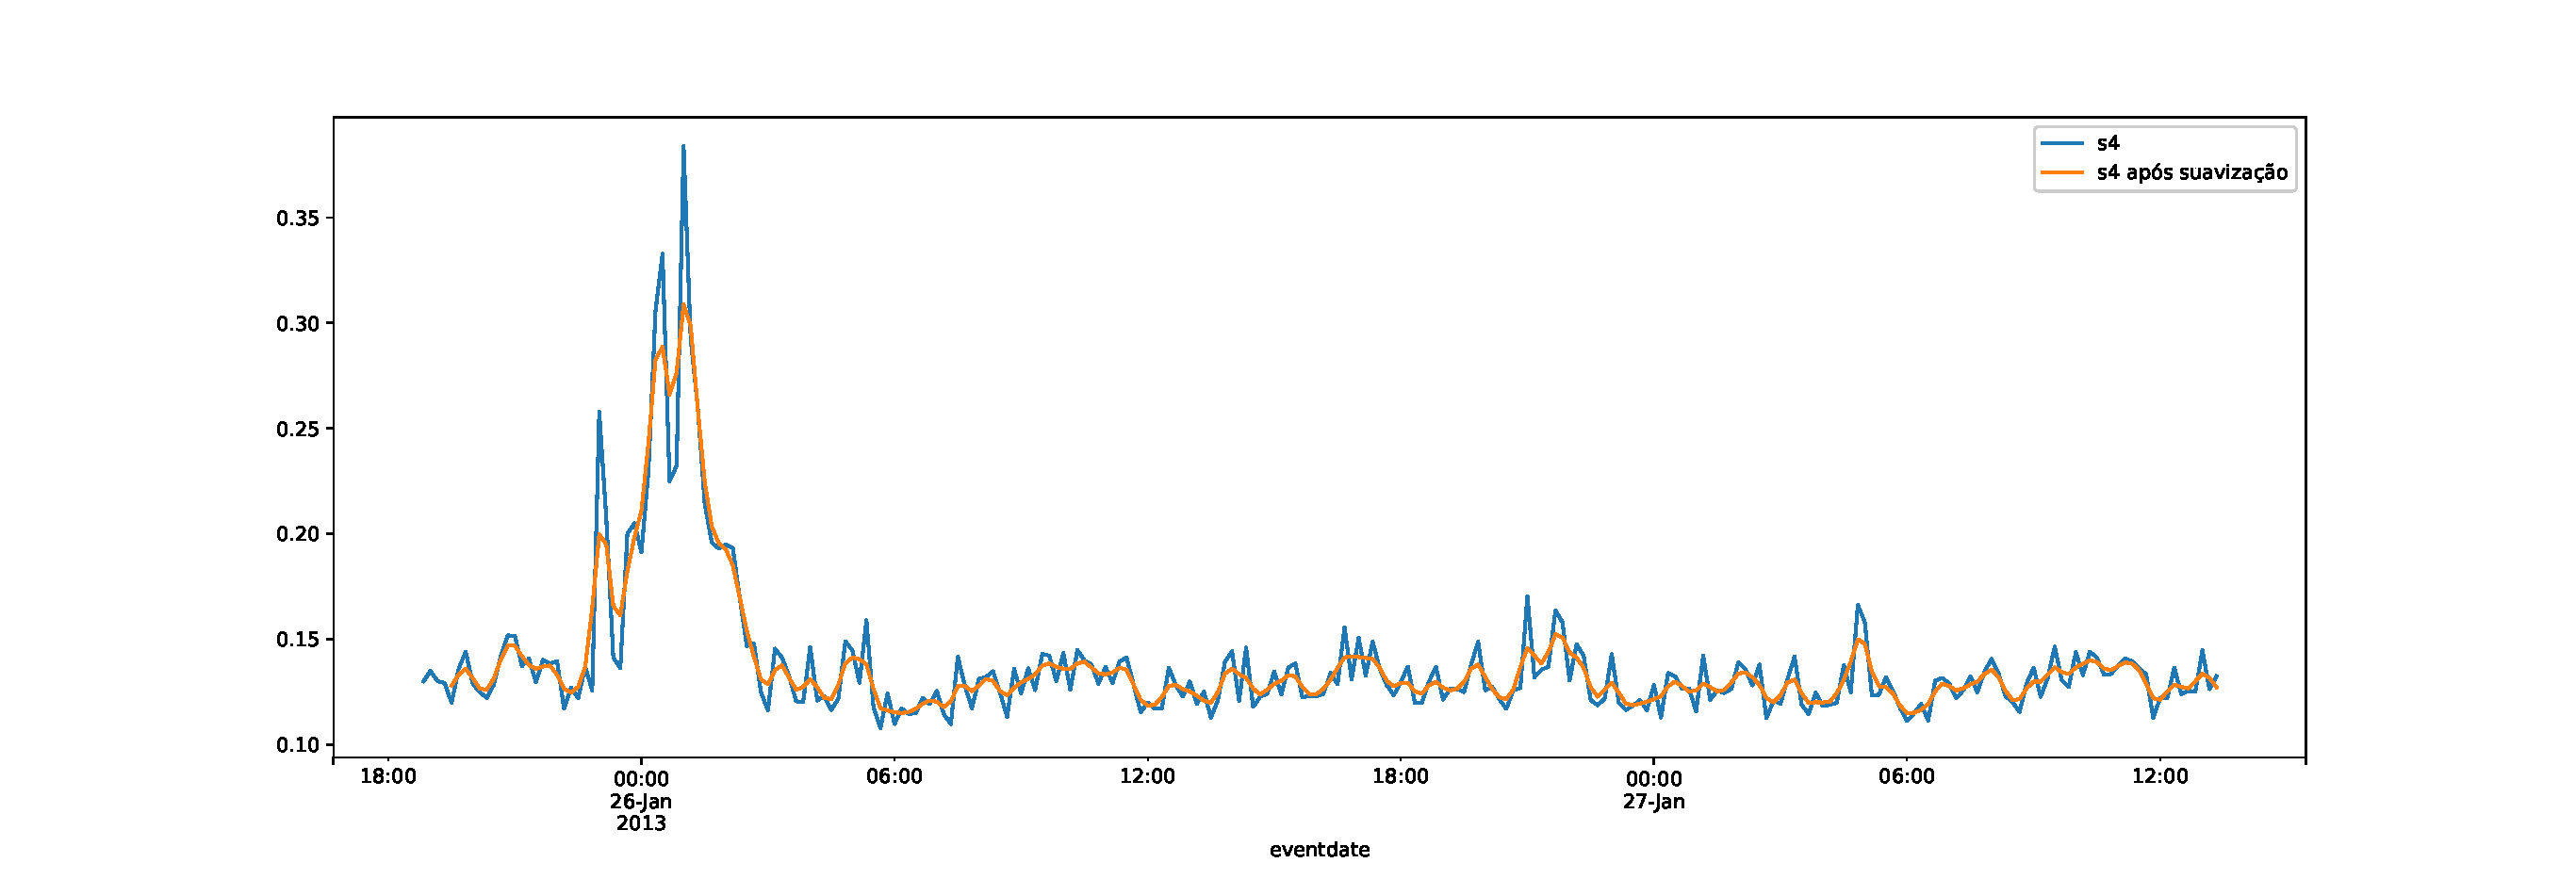
\includegraphics[width=1.4\linewidth]{./Figuras/s4_signal_noise_and_smooth_gaussian.eps}}
\caption{Suavização de uma amostra da série temporal de S4, por meio de uma média móvel com peso gaussiano.}
\label{fig:gaussian}
\end{figure}

Finalmente, optou-se por utilizar uma combinação das duas técnicas de suavização aplicando primeiro do filtro de Savitzky–Golay seguido da média móvel com pesos gaussianos, ambos com os parâmetros especificados no parágrafo anterior. Essa escolha gera um sinal mais suave do que a aplicação de um ou outro.

Este notebook gera também uma tabela com todos os dados de S4, em passos de 10 min, onde as colunas representam o conjunto inicial de estações.

\section{Extração da série temporal de VTEC, para algumas estações}

O papel do notebook 03\_extract\_vtec\_stations.ipynb é o de extrair séries temporais da série espaço-temporal do VTEC, para localizações em que existam estações onde o índice S4 é medido. Estes dados então são preprocessados aplicando o mesmo processo de suavização utilizados nos dados de cintilação. Na figura \ref{fig:vtecsj2} é possível visualizar uma amostra do VTEC para São José dos Campos, juntamente com a aplicação das duas técnicas de suavização. Na figura \ref{fig:vtecsignal} há uma amostra do sinal de VTEC para o conjunto inicial de estações, observe que no intervalo entre às 9:00 e 15:00 UT o VTEC é aproximadamente similar entre as diversas estações, e que a partir das 18:00 UT os valores começam a divergir entre si, apresentado grandes diferenças após 00:00 UT, até 06:00 UT, onde então começam a se agrupar. Tal padrão se apresenta ao longo de todo o período amostrado para este trabalho.

\begin{figure}[H]
\centering
\makebox[\textwidth][c]{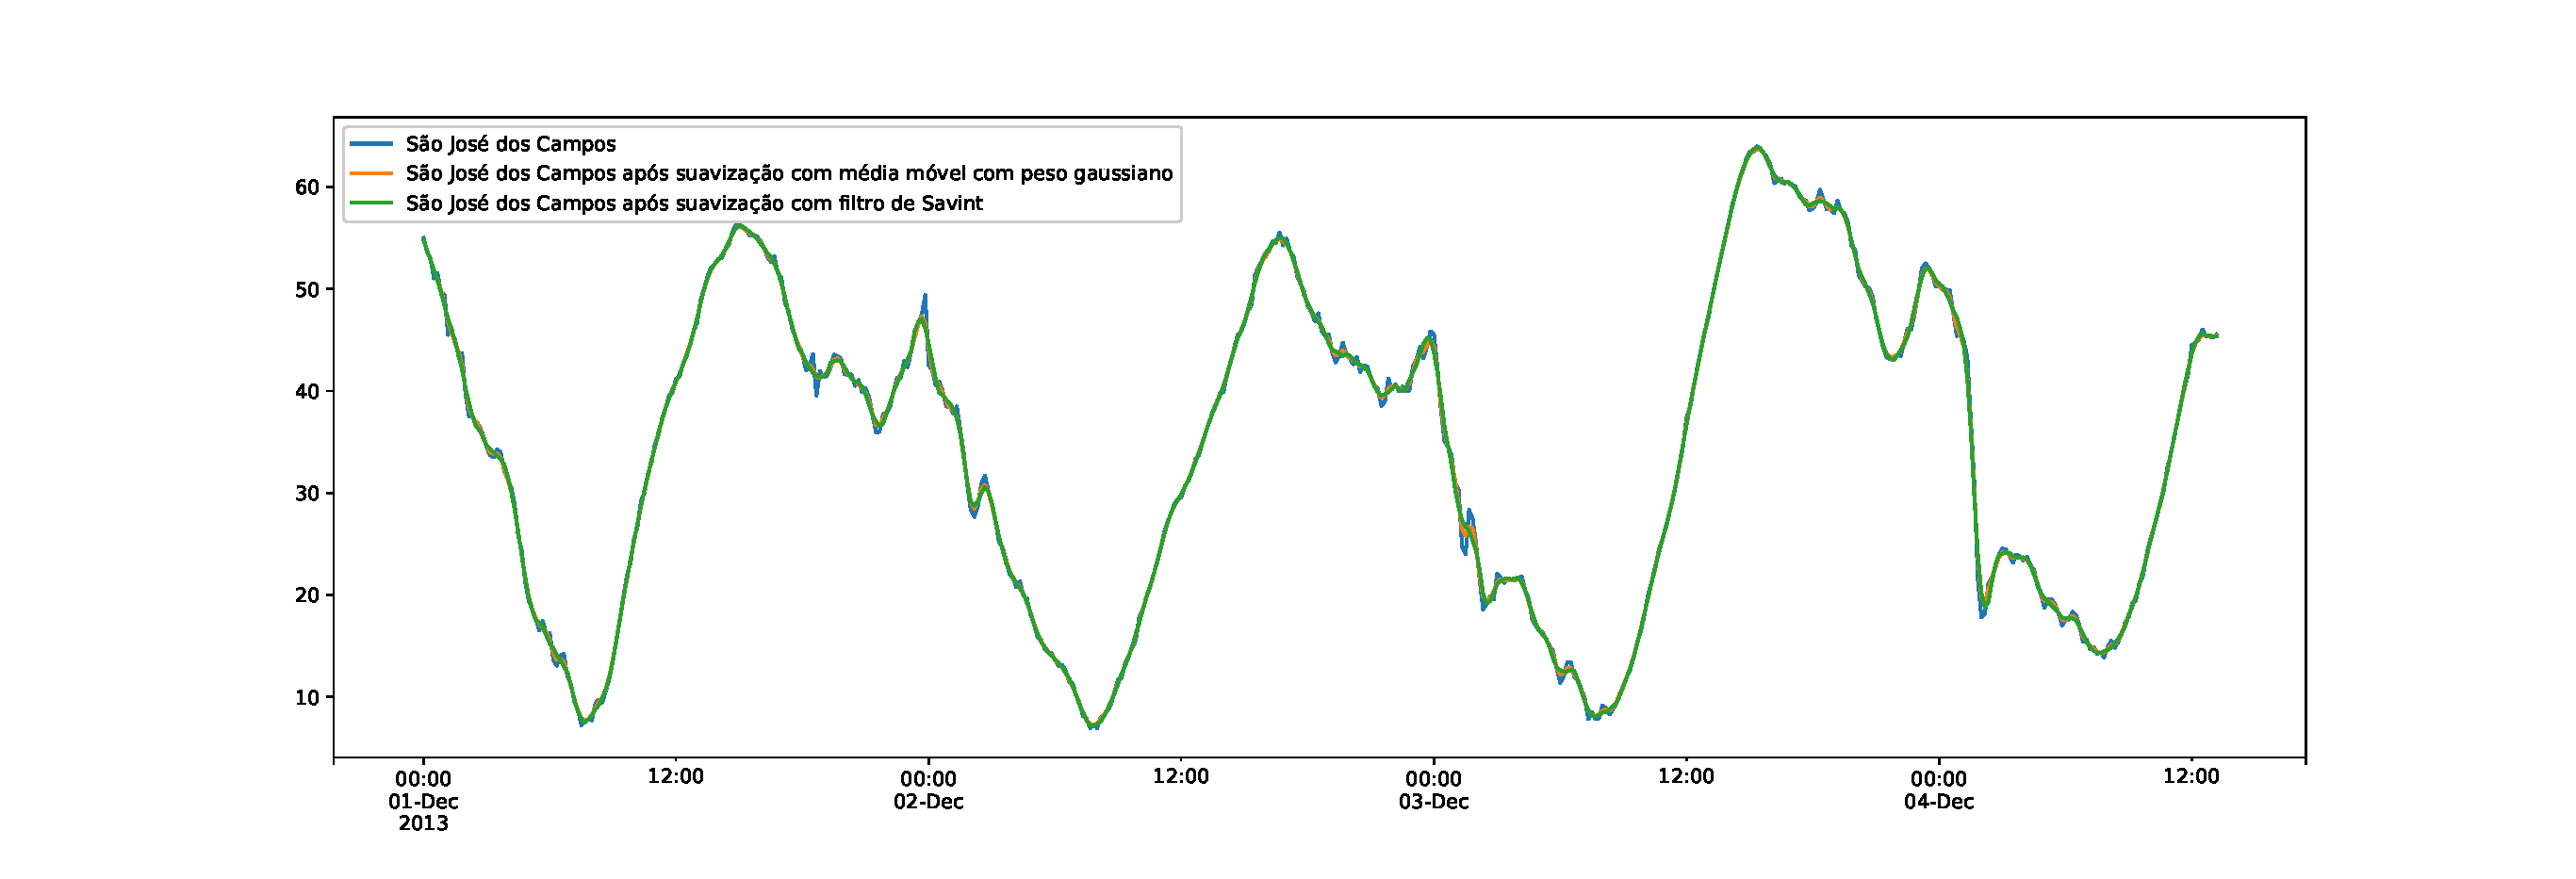
\includegraphics[width=1.5\columnwidth]{./Figuras/vtec_sj2.eps}}
\caption{Amostra de um sinal de VTEC, juntamente com suas suavizações pelo método Savitzky–Golay e média móvel com peso gaussiano.}
\label{fig:vtecsj2}

\makebox[\textwidth][c]{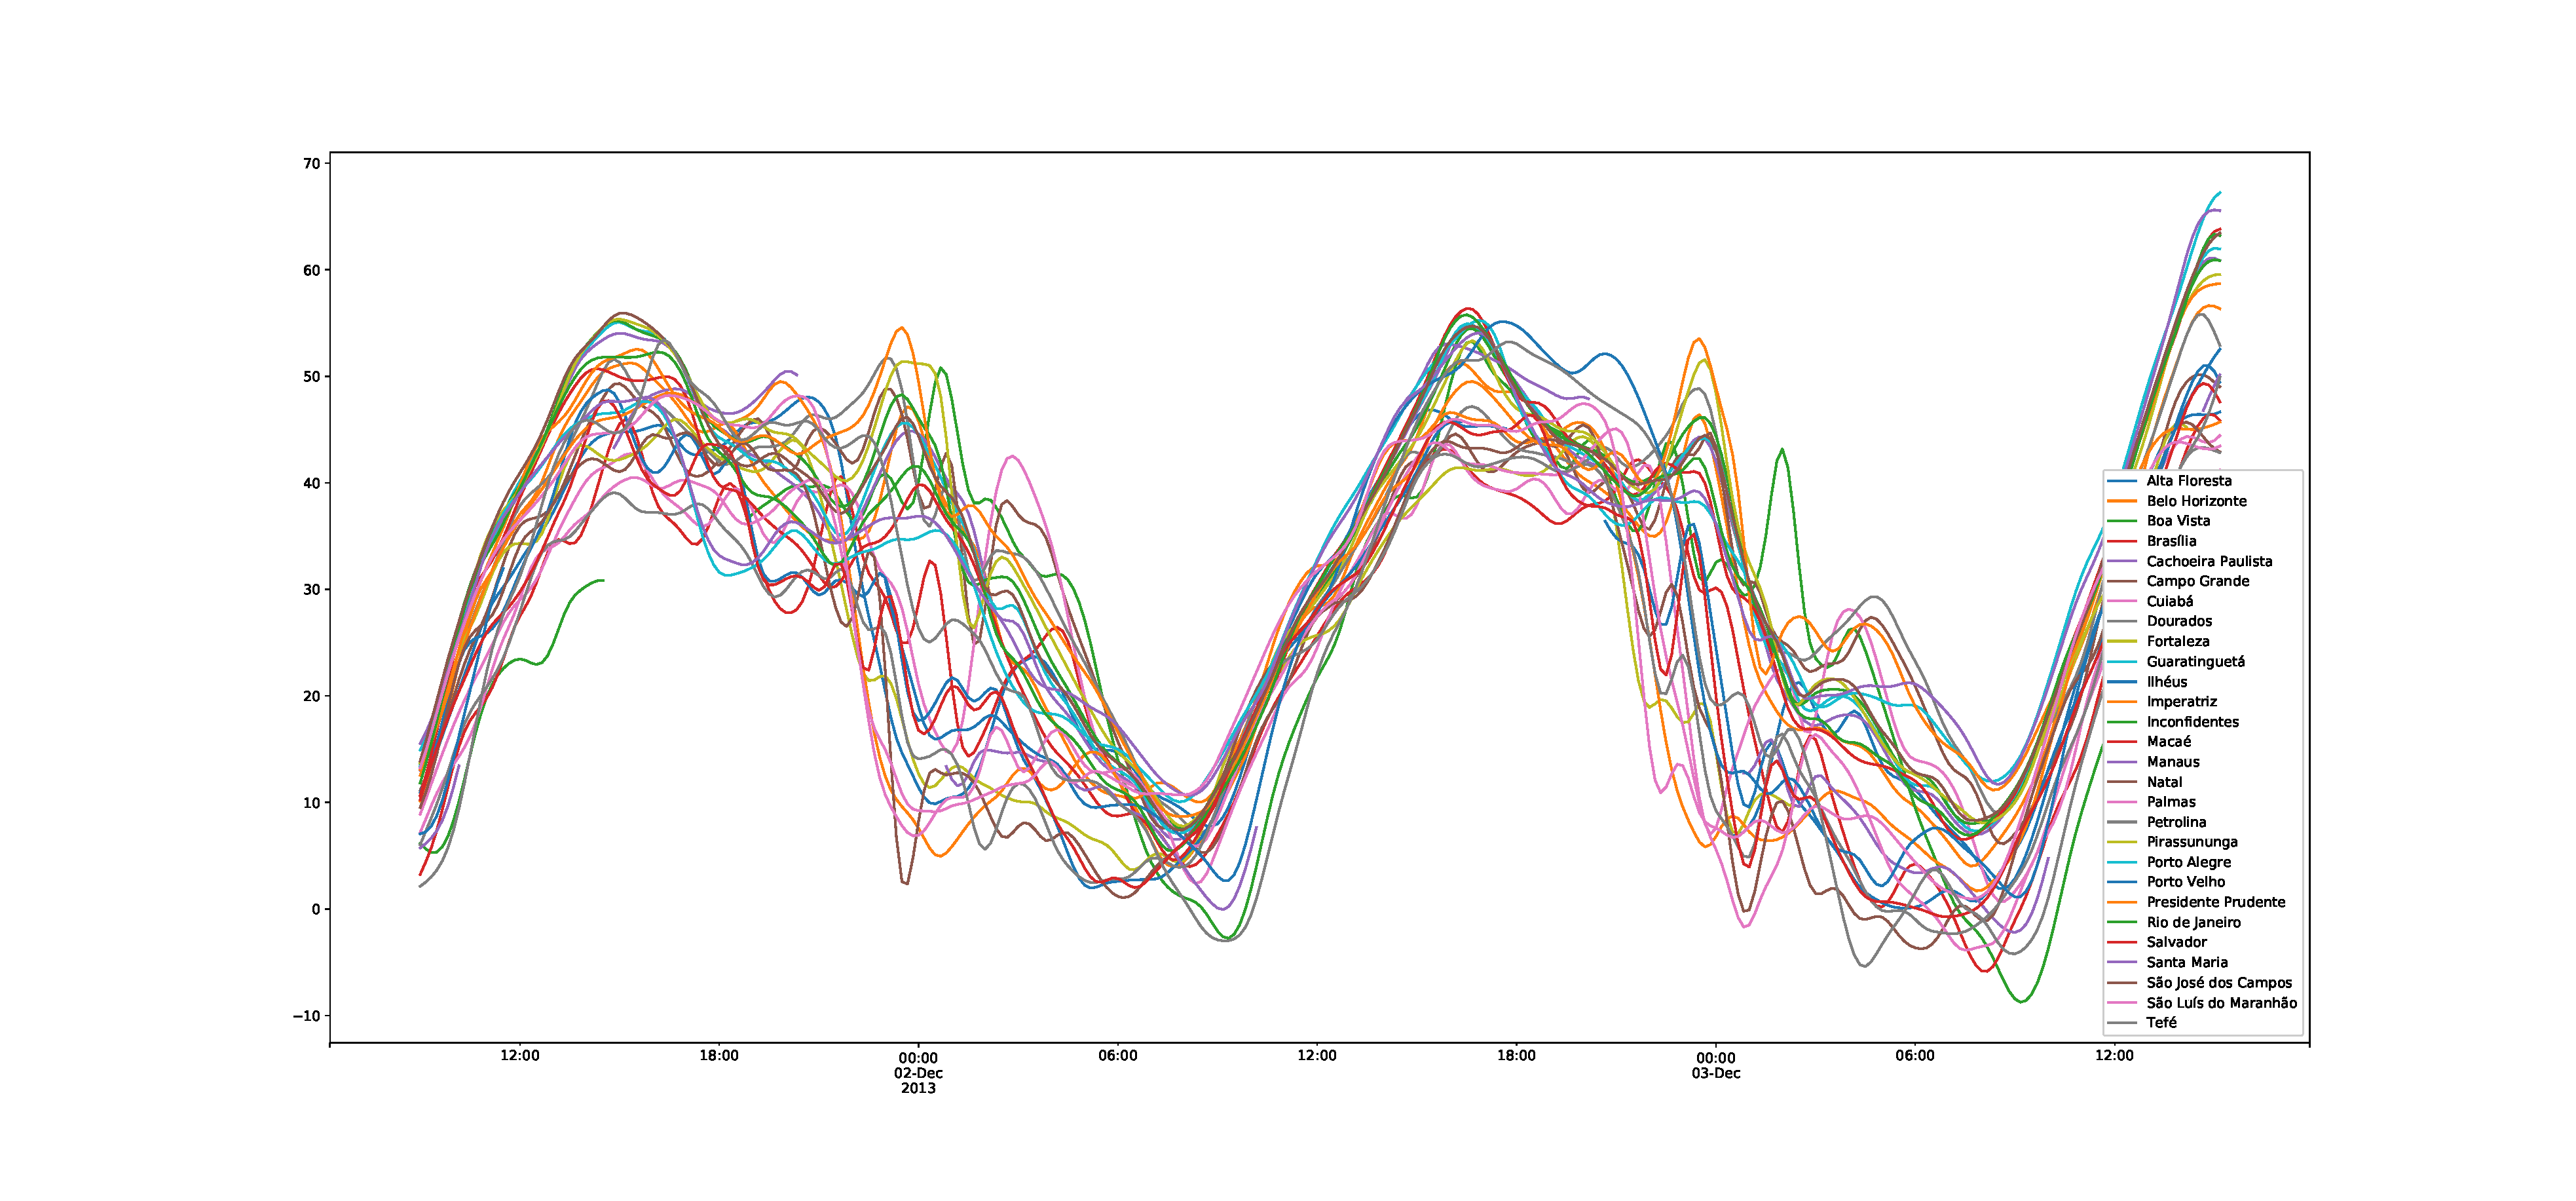
\includegraphics[width=1.5\columnwidth]{./Figuras/vtec_signal.eps}}
\caption{Amostra de um sinal de VTEC, para múltiplas estações. Note a convergência da série para a vizinhança das 12:00 UT e sua divergência próximo das 00:00 UT.}
\label{fig:vtecsignal}
\end{figure}

Em sua fase final este notebook gera uma tabela, onde cada coluna representa uma estação diferente com os dados de VTEC indexados pelo tempo, de modo que, pode-se falar em uma tabela de séries temporais para os dados de VTEC.

\section{Seleção fina dos dados de S4}

Após o pré-processamento dos dados de S4, é realizada uma seleção mais fina das estações que serão utilizadas neste trabalho, para tal foi empregado o notebook 04\_reanalize\_data.ipynb. O primeiro conjunto de estações descartas o foi, pois apresentava poucos pontos ao longo do período de janeiro de 2013 à dezembro de 2014 o que levou a curvas interpoladas que não são condizentes com a variável observada, o que foi evidenciado pela plotagem das séries temporais. 

Os dados de VTEC foram amostrados em um intervalo menor do que o S4, assim, foi realizado um recorte na série temporal de S4, tal que ambas as séries tenham o mesmo intervalo de amostragem. Assim, o segundo conjunto de estações descartadas são aquelas que não apresentam medidas no período de tempo selecionado. A tabela \ref{tab:stations} apresenta o grupo final de estações selecionados para o trabalho. As figuras \ref{fig:s4stations0}, \ref{fig:s4stations1} e \ref{fig:s4stations2} exibem a série temporal S4 para este grupo de estações, enquanto a figura \ref{fig:mapstationsre} apresenta um mapa com estas.

\begin{table}
\addtolength{\leftskip} {-2cm} % increase (absolute) value if needed
\addtolength{\rightskip}{-2cm}
\small
\begin{tabular}{|l|l|l|c|c|c|c|c|}
\hline
Cidade              & Est.  & Cód. de Id.           &  Alt.     &   Lat.     &  Lon.      &  Lat. Mag.    &  Lon. Mag.       \\ \hline
Belo Horizonte      &    MG &                   bhz &   858.000 & -19.868500 & -43.954200 &    -25.426147 &      24.786619   \\ \hline
Brasília            &    DF &                   bsa &  1050.000 & -15.764200 & -47.869400 &    -24.348659 &      22.352744   \\ \hline
Cachoeira Paulista  &    SP &                   cpa &   580.000 & -22.410000 & -45.000000 &    -24.456556 &      22.960540   \\ \hline
Campo Grande        &    MS &                    32 &       NaN & -20.497000 & -54.615000 &    -21.417704 &      14.873907   \\ \hline
Cuiabá              &    MT &                   cub &   278.000 & -15.555200 & -56.069800 &    -14.336068 &      14.530440   \\ \hline
Dourados            &    MS &                   dou &   756.120 & -22.110000 & -54.550000 &    -23.627266 &      14.698554   \\ \hline
Fortaleza           &    CE &                    24 &       NaN &  -3.742000 & -38.539000 &           NaN &            NaN   \\ \hline
Guaratinguetá       &    SP &                    33 &       NaN & -22.789000 & -45.220000 &    -24.188879 &      22.620120   \\ \hline
Ilhéus              &    BA &                   ios &     0.000 & -14.470000 & -39.100000 &    -13.470248 &      30.548727   \\ \hline
Inconfidentes       &    MG &                    25 &       NaN & -22.318000 & -46.329000 &    -26.299459 &      22.004117   \\ \hline
Macaé               &    RJ &                    11 &       NaN & -22.823000 & -41.785700 &    -20.542047 &      25.191448   \\ \hline
Natal               &    RN &                   nta &     0.000 &  -5.836162 & -35.121000 &           NaN &            NaN   \\ \hline
Palmas              &    RO &                     3 &       NaN & -10.200000 & -48.312000 &    -12.264838 &      23.425112   \\ \hline
Pirassununga        &    SP &                    30 &       NaN & -21.989000 & -47.334000 &    -23.990783 &      21.003125   \\ \hline
Porto Alegre        &    RS &                     4 &       NaN & -30.071000 & -51.119000 &    -22.954879 &      15.550843   \\ \hline
Presidente Prudente &    SP &                     6 &       NaN & -22.120000 & -51.407000 &    -21.640946 &      17.249042   \\ \hline
Rio de Janeiro      &    RJ &                    34 &       NaN & -22.823000 & -43.238000 &    -20.105803 &      23.888647   \\ \hline
Salvador            &    BA &                    26 &       NaN & -13.001000 & -38.508000 &    -12.123350 &      31.680944   \\ \hline
Santa Maria         &    RS &                   sta &   110.100 & -29.712591 & -53.717206 &    -22.659740 &      13.628064   \\ \hline
São José dos Campos &    SP &                   sj2 &   593.440 & -23.207000 & -45.859000 &    -24.835610 &      22.002028   \\ \hline
Tefé                &    AM &                   tfe &     0.057 &  -3.180000 & -64.440000 &      6.385157 &       9.314963   \\ \hline
\end{tabular}\label{tab:stations}

\vspace{12pt}

\begin{center}
\begin{tabular}{|l|c|c|c|}
\hline
Cidade              &   Alt. da Cidade &  Lat. da Cidade &  Lon. da Cidade \\ \hline
Belo Horizonte      &            767.0 &       -19.81570 &        -43.9542 \\ \hline
Brasília            &           1130.0 &       -15.78010 &        -47.9292 \\ \hline
Cachoeira Paulista  &            545.0 &       -22.67370 &        -44.9973 \\ \hline
Campo Grande        &            612.0 &       -20.44350 &        -54.6478 \\ \hline
Cuiabá              &            180.0 &       -15.59890 &        -56.0949 \\ \hline
Dourados            &            448.0 &       -22.22180 &        -54.8064 \\ \hline
Fortaleza           &             14.0 &        -3.71839 &        -38.5434 \\ \hline
Guaratinguetá       &            526.0 &       -22.81620 &        -45.1935 \\ \hline
Ilhéus              &              9.0 &       -14.79730 &        -39.0355 \\ \hline
Inconfidentes       &            864.0 &       -22.31710 &        -46.3284 \\ \hline
Macaé               &              7.0 &       -22.37170 &        -41.7857 \\ \hline
Natal               &             38.0 &        -5.79448 &        -35.2110 \\ \hline
Palmas              &            260.0 &       -10.16890 &        -48.3317 \\ \hline
Pirassununga        &            625.0 &       -21.99600 &        -47.4268 \\ \hline
Porto Alegre        &             22.0 &       -30.02770 &        -51.2287 \\ \hline
Presidente Prudente &            471.0 &       -22.12760 &        -51.3856 \\ \hline
Rio de Janeiro      &             20.0 &       -22.90350 &        -43.2096 \\ \hline
Salvador            &             12.0 &       -12.97040 &        -38.5124 \\ \hline
Santa Maria         &            139.0 &       -29.69140 &        -53.8008 \\ \hline
São José dos Campos &            593.0 &       -23.17910 &        -45.8872 \\ \hline
Tefé                &             28.0 &        -3.32073 &        -64.7236 \\ \hline
\end{tabular}
\end{center}

\vspace{12pt}

\caption{Conjunto de estações que realizam medidas do índice S4 juntamente com seus atributos.}
\label{tab:stations}
\end{table}

\begin{figure}[H]
\centering
\makebox[\textwidth][c]{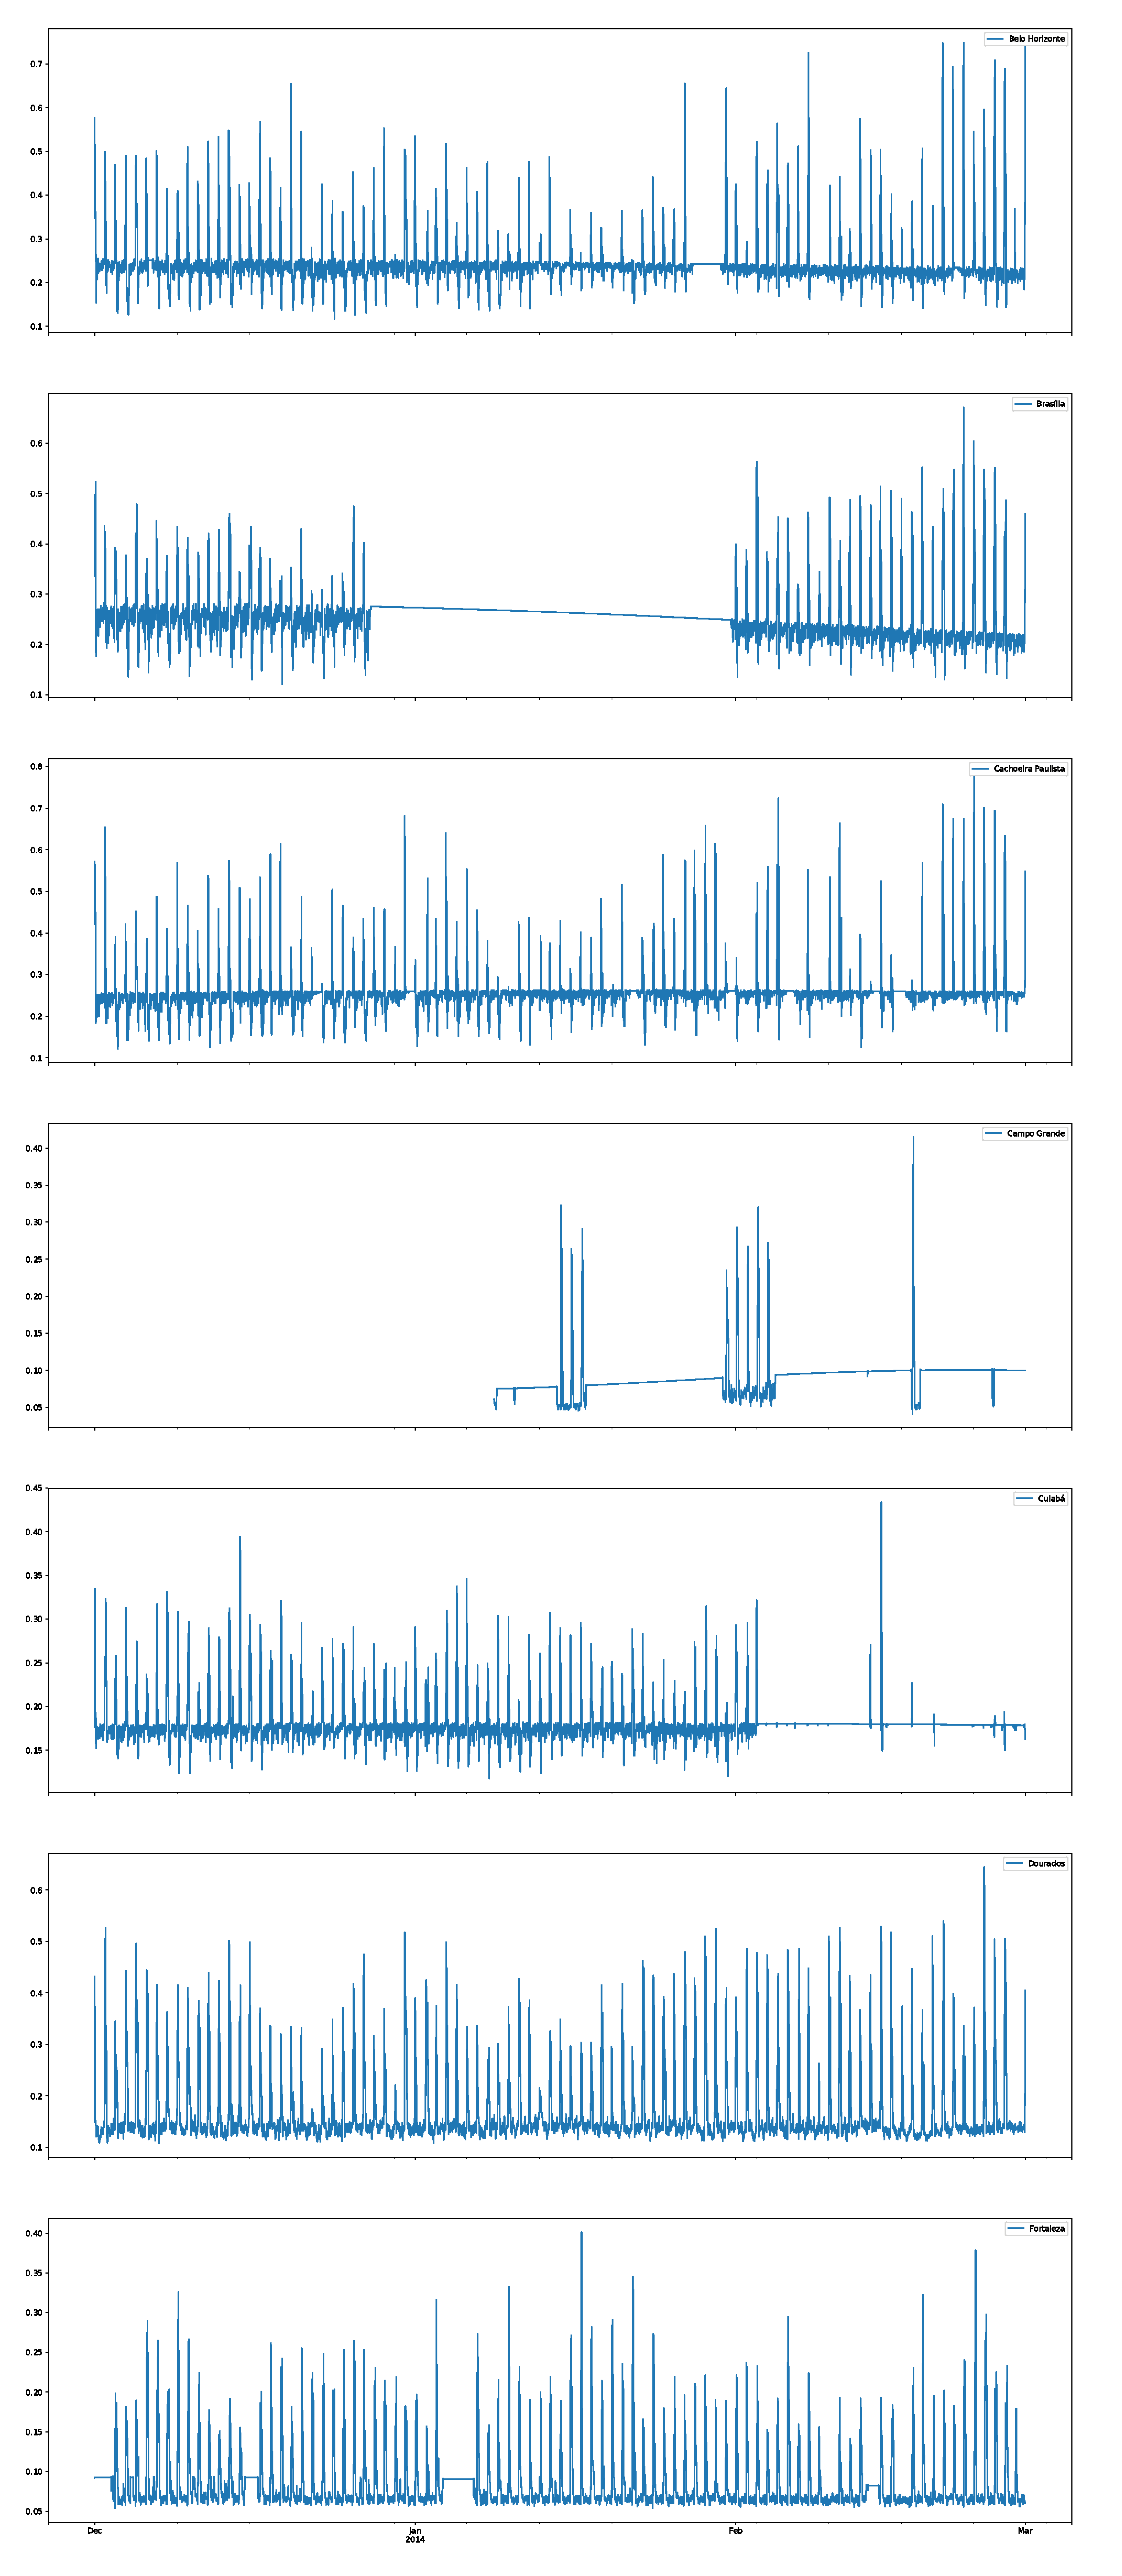
\includegraphics[width=1.0\columnwidth]{./Figuras/s4_stations0.eps}}
\label{fig:s4stations0}
\caption{Amostra do sinal S4 para o primeiro subconjunto de estações.}
\end{figure}

\begin{figure}[H]
\centering
\makebox[\textwidth][c]{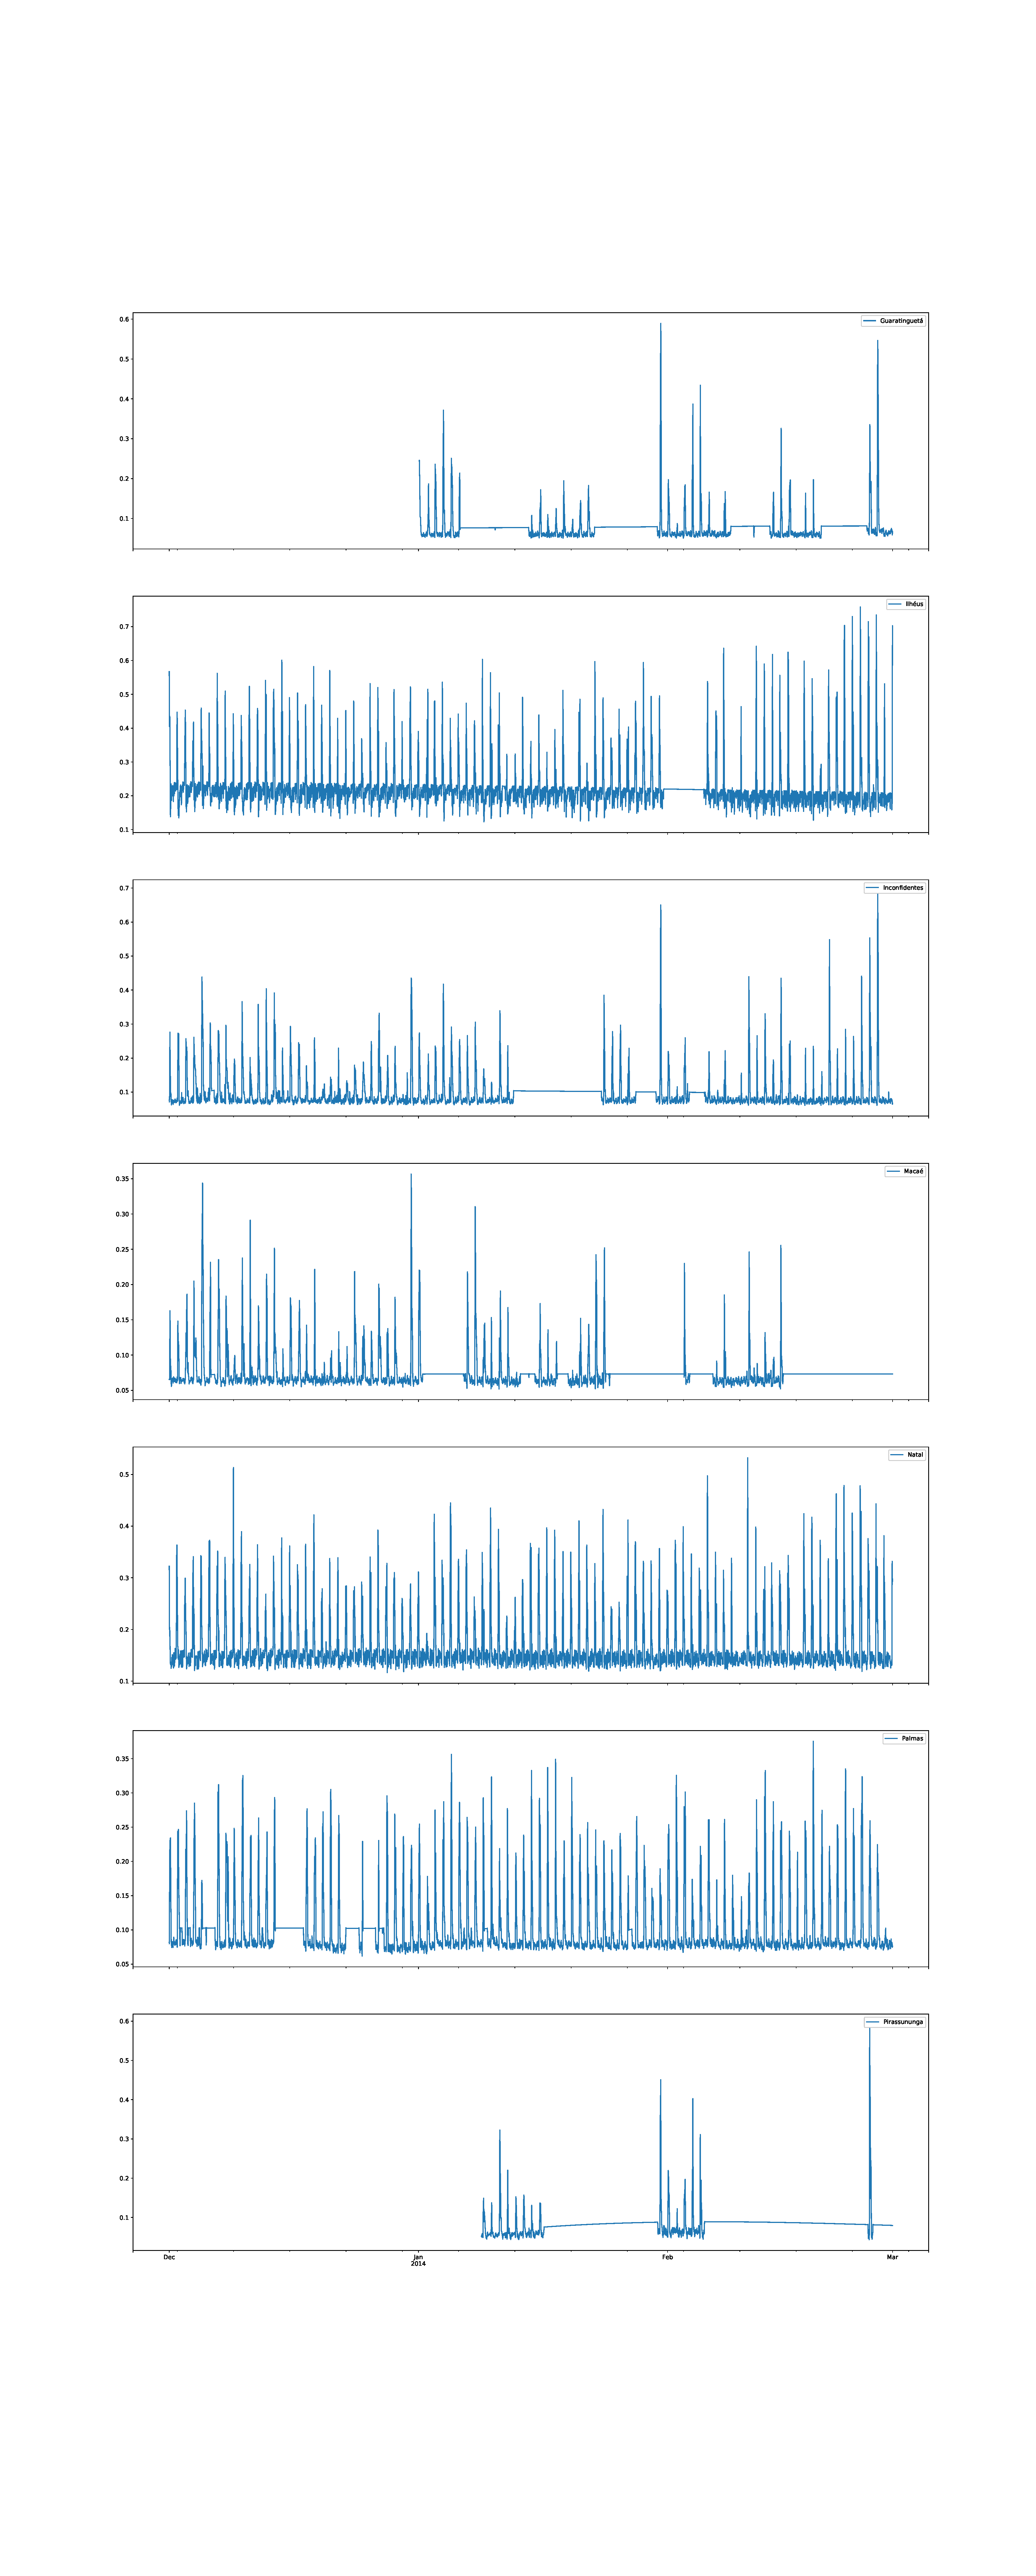
\includegraphics[width=1.5\columnwidth]{./Figuras/s4_stations1.eps}}
\label{fig:s4stations1}
\caption{Amostra do sinal S4 para o segundo subconjunto de estações.}
\end{figure}

\begin{figure}[H]
\centering
\makebox[\textwidth][c]{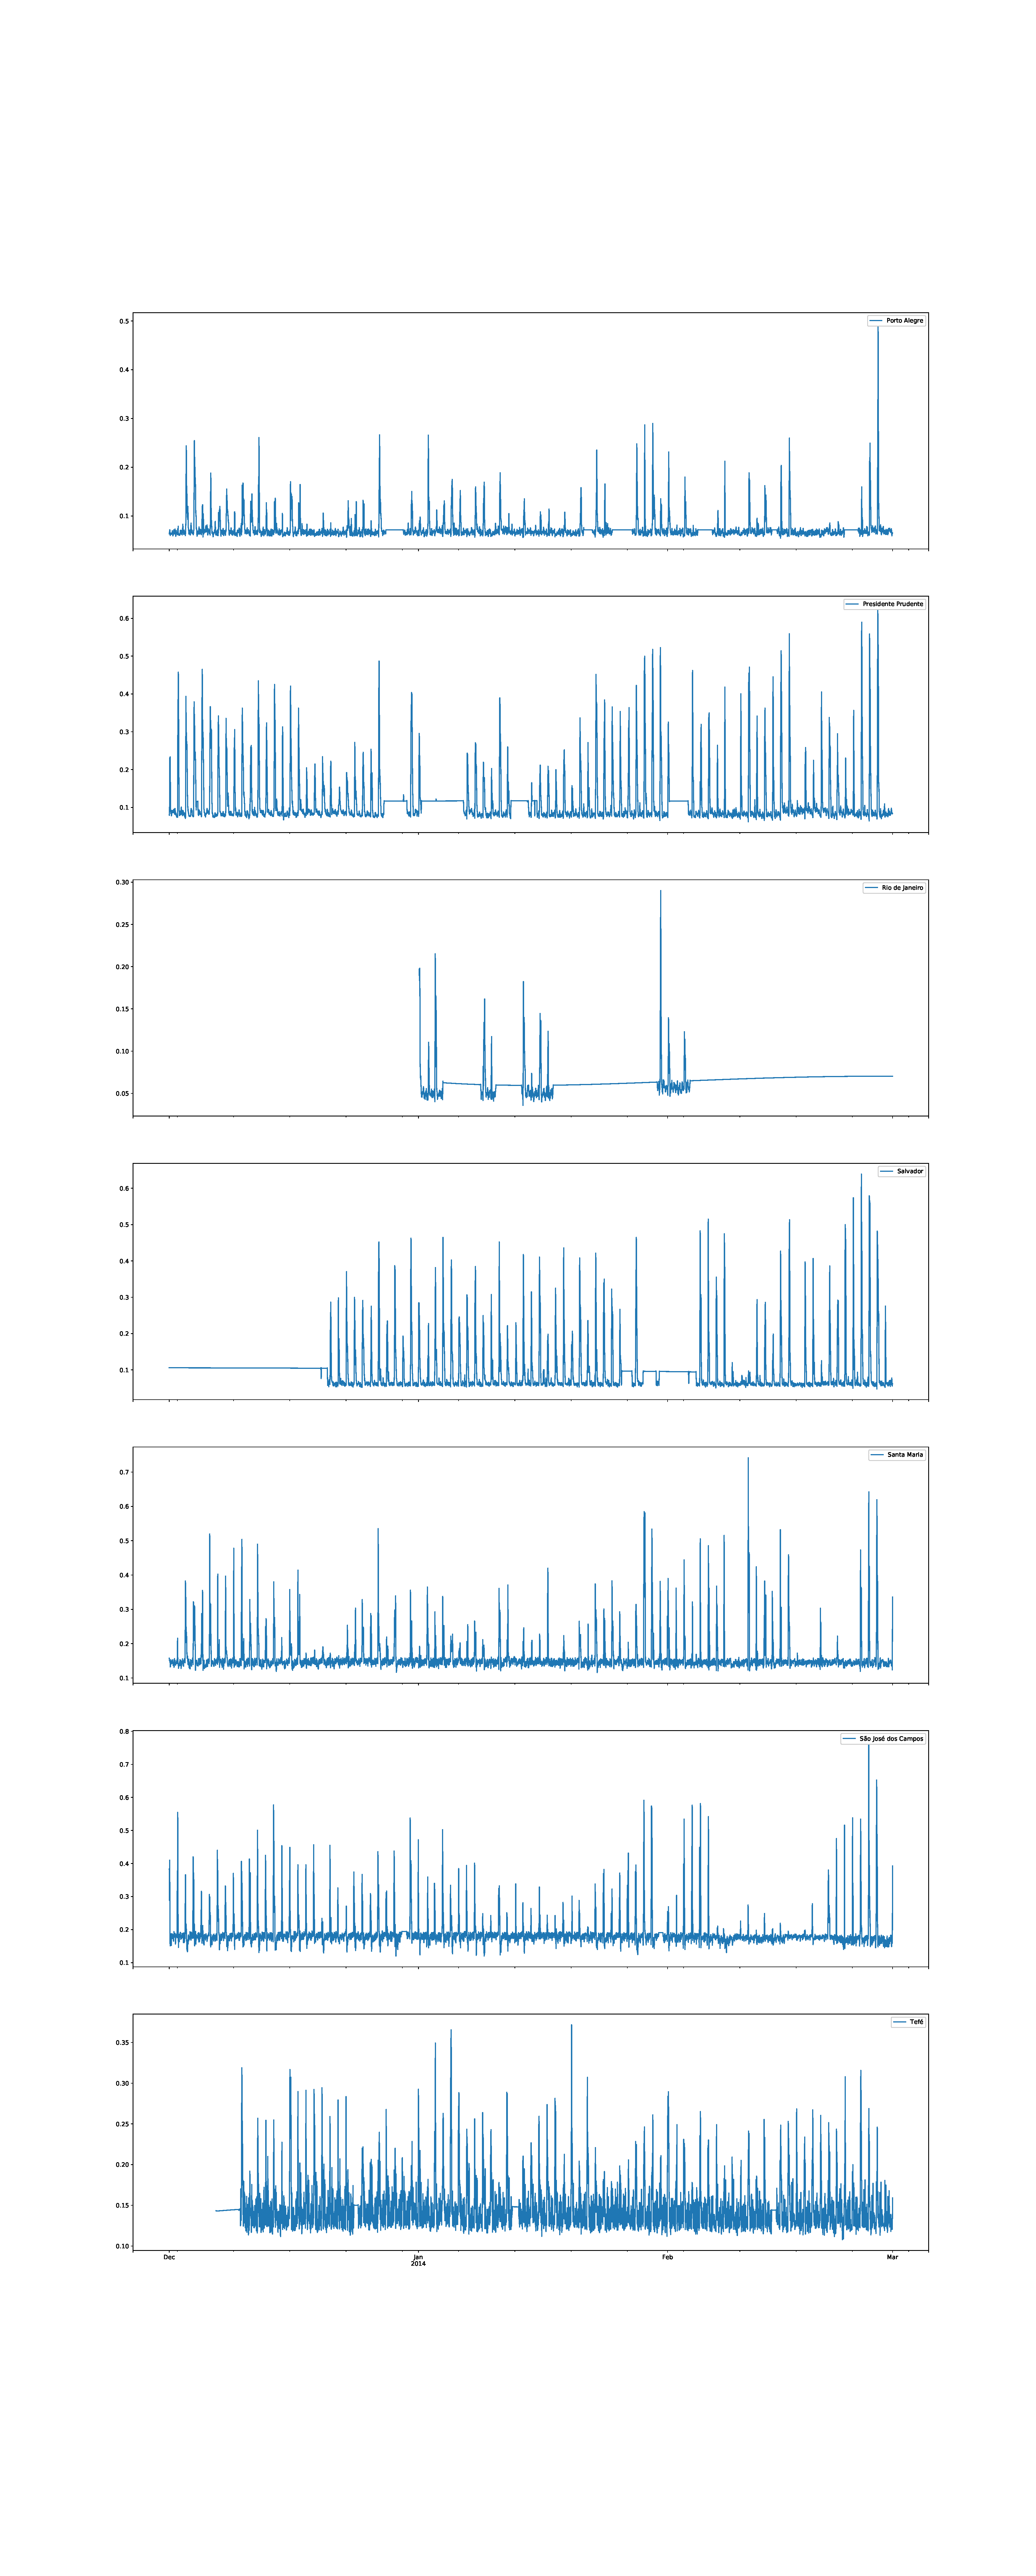
\includegraphics[width=1.5\columnwidth]{./Figuras/s4_stations2.eps}}
\label{fig:s4stations2}
\caption{Amostra do sinal S4 para o terceiro subconjunto de estações.}
\end{figure}

\begin{figure}[h]
\centering
\makebox[\textwidth][c]{\includesvg[width=1.6\columnwidth]{./Figuras/map_stations_re.svg}}
\label{fig:mapstationsre}
\caption{Conjunto final de estações que serão utilizadas para este trabalho.}
\end{figure}

\section{Visualizando S4  e VTEC}\label{sec:viss4vtec}

Feita uma seleção mais fina das estações que fornecem as séries temporais de S4, assim, como um recorte adequado no tempo, é adequado plotar a série temporal do VTEC, juntamente com a do S4. Esta etapa é realizada no notebook 05\_visualize\_vtec\_s4\_data. Os gráficos são feitos em dois grupos distintos, o primeiro apresenta uma amostra das séries temporais, fornecendo um resolução visual melhor, enquanto o segundo fornece a série completa. Algumas observações pode ser feitas analisando visualmente ambos os conjuntos. Nota-se, por exemplo:

\begin{itemize}
\item uma periodicidade em ambos os dados; 
\item os valores de S4 sobem conforme o do VTEC diminui;
\item os valores de pico de S4 aparecem em quedas e mínimos do VTEC;
\item os dados de S4 apresentam maior ruído e menor disponibilidade;
\item flutuações mais intensas do S4 aparecem no máximo do VTEC.
\end{itemize}

\begin{figure}[H]
\centering
\makebox[\textwidth][c]{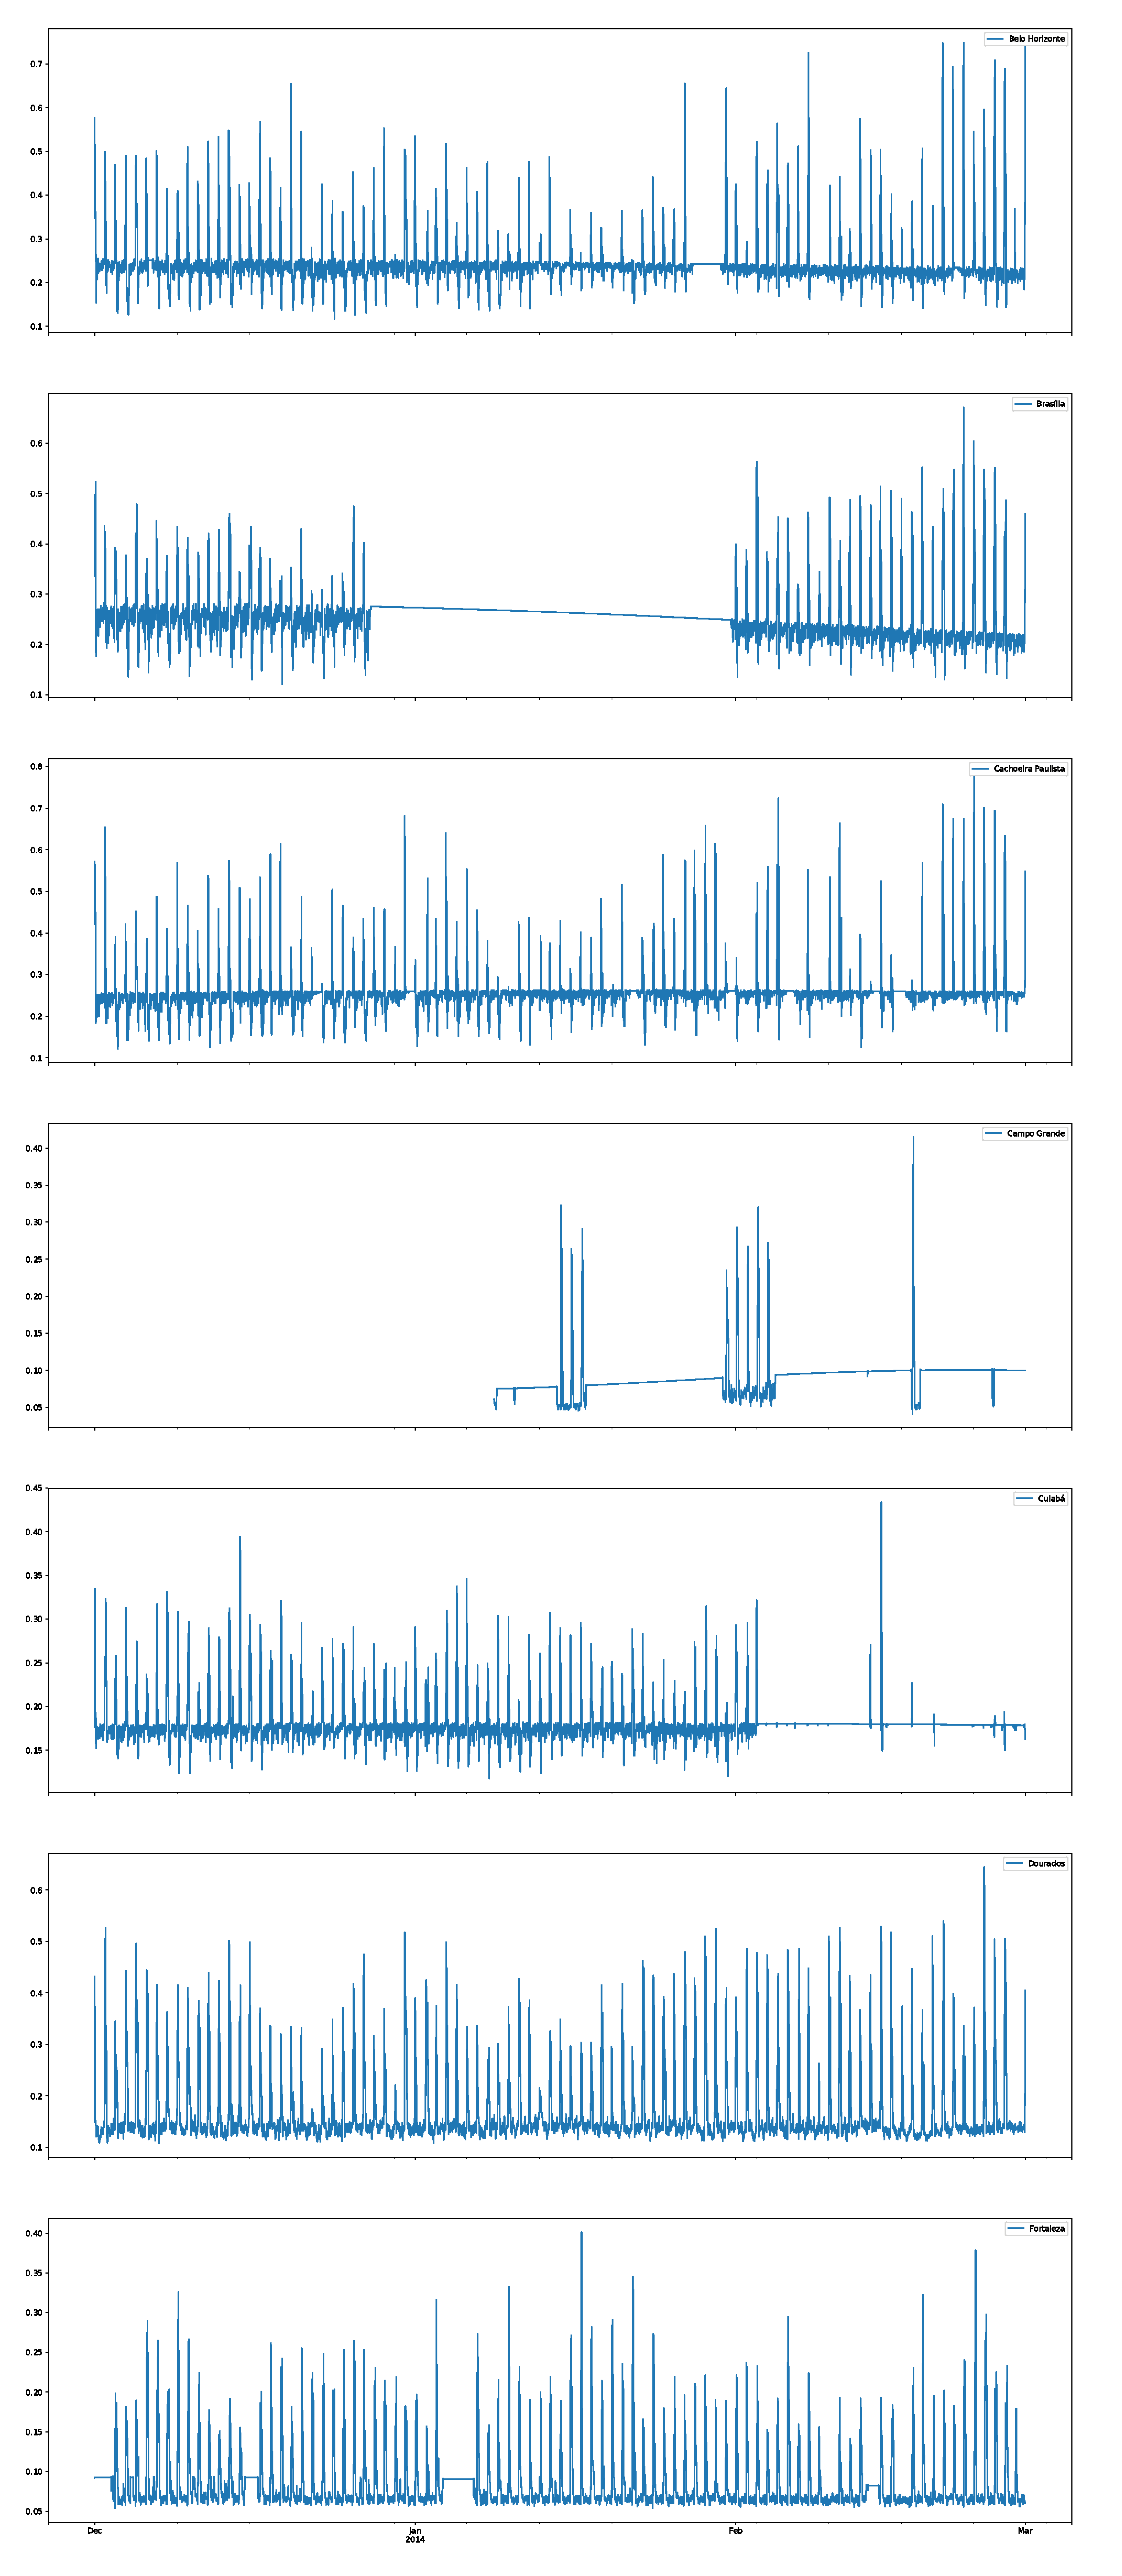
\includegraphics[width=1.0\columnwidth]{./Figuras/s4_stations0.eps}}
\label{fig:s4stations0}
\caption{Amostra do sinal S4 para o primeiro subconjunto de estações.}
\end{figure}

\begin{figure}[H]
\centering
\makebox[\textwidth][c]{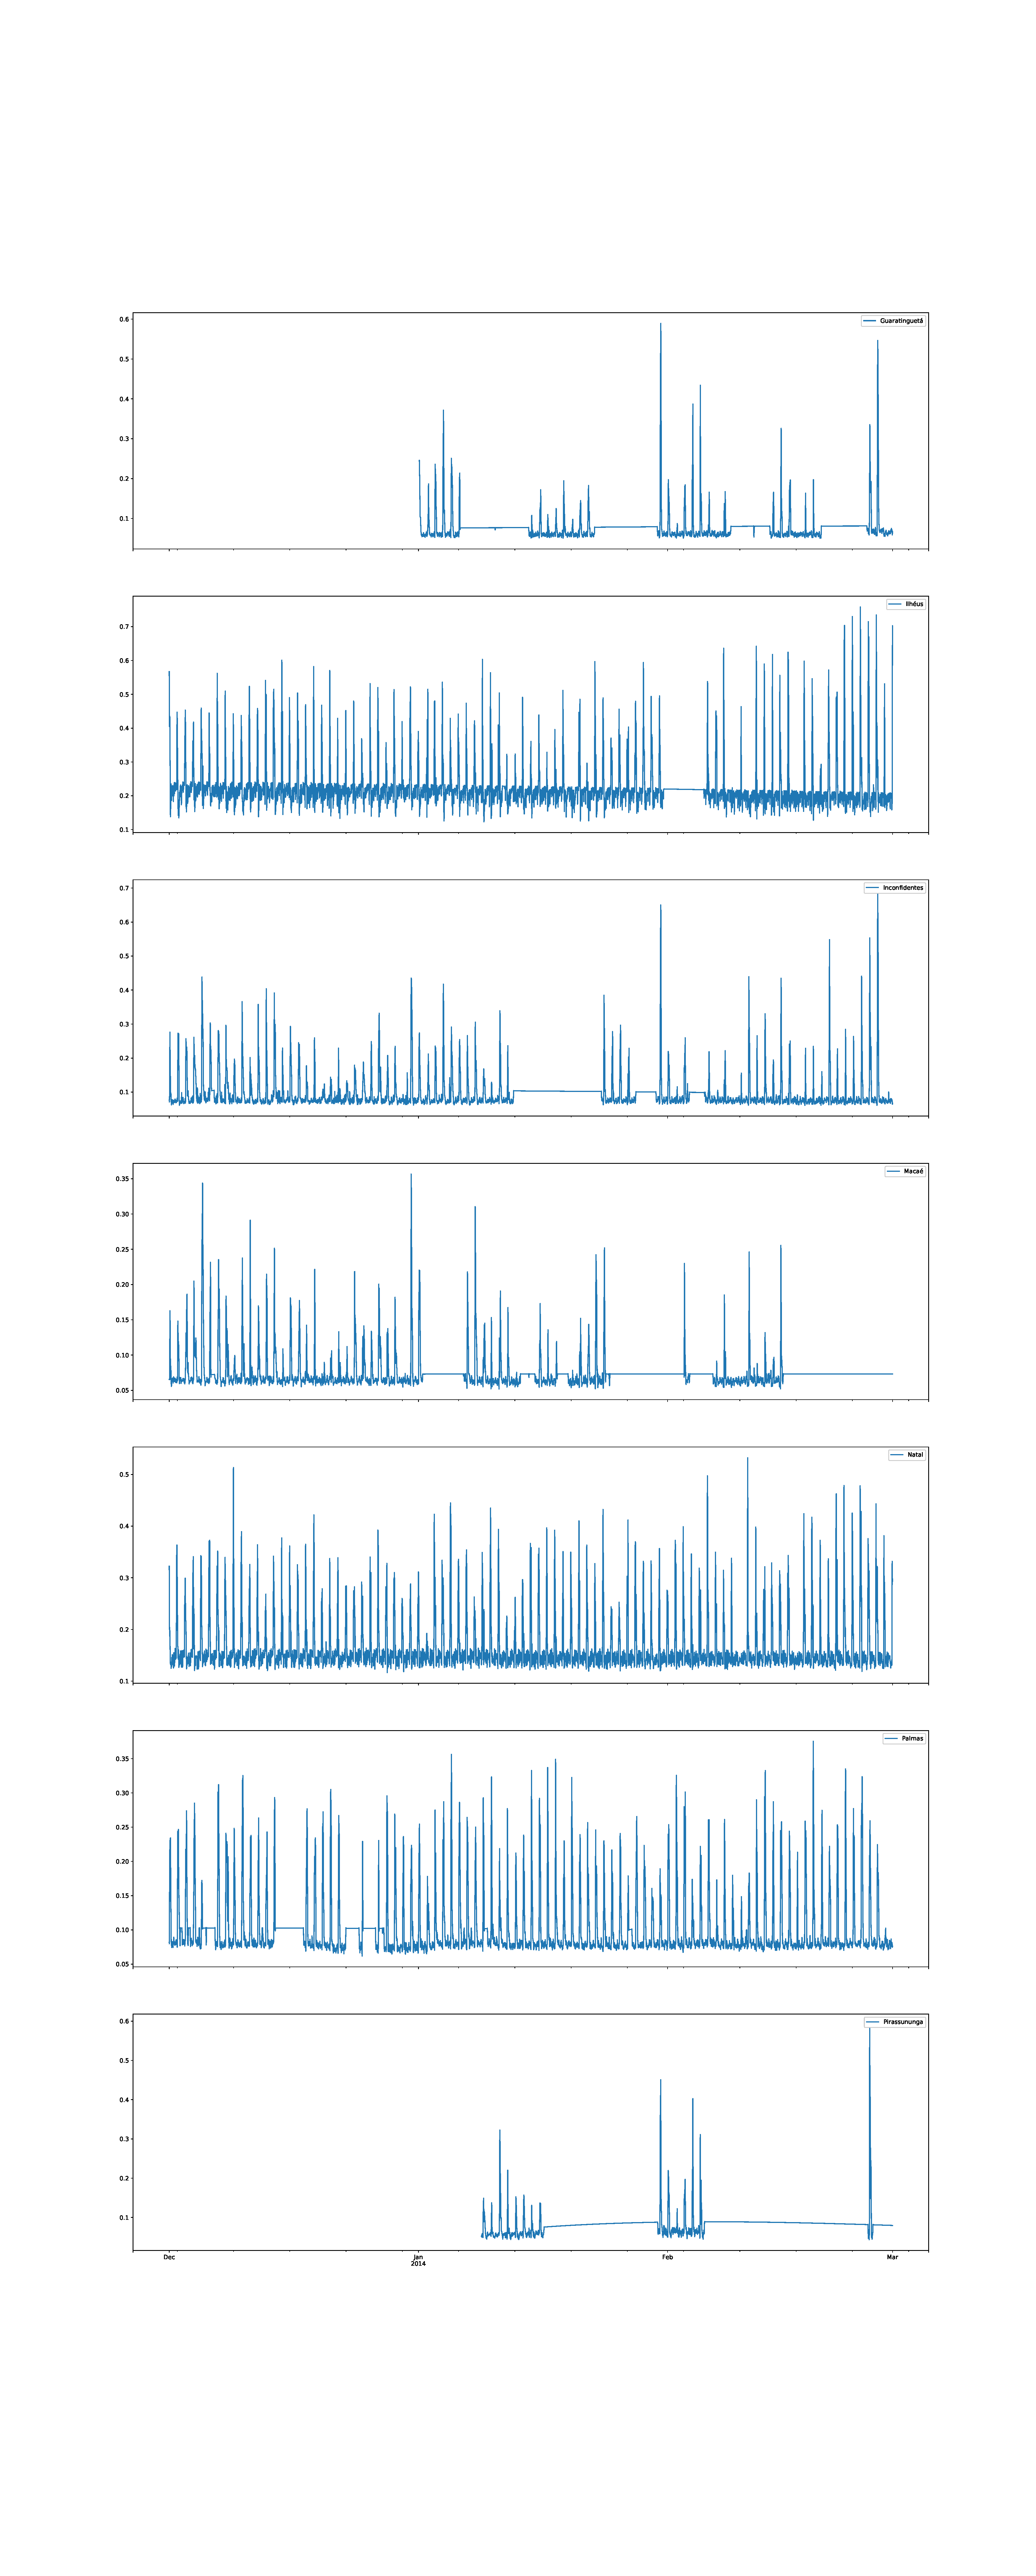
\includegraphics[width=1.5\columnwidth]{./Figuras/s4_stations1.eps}}
\label{fig:s4stations1}
\caption{Amostra do sinal S4 para o segundo subconjunto de estações.}
\end{figure}

\begin{figure}[H]
\centering
\makebox[\textwidth][c]{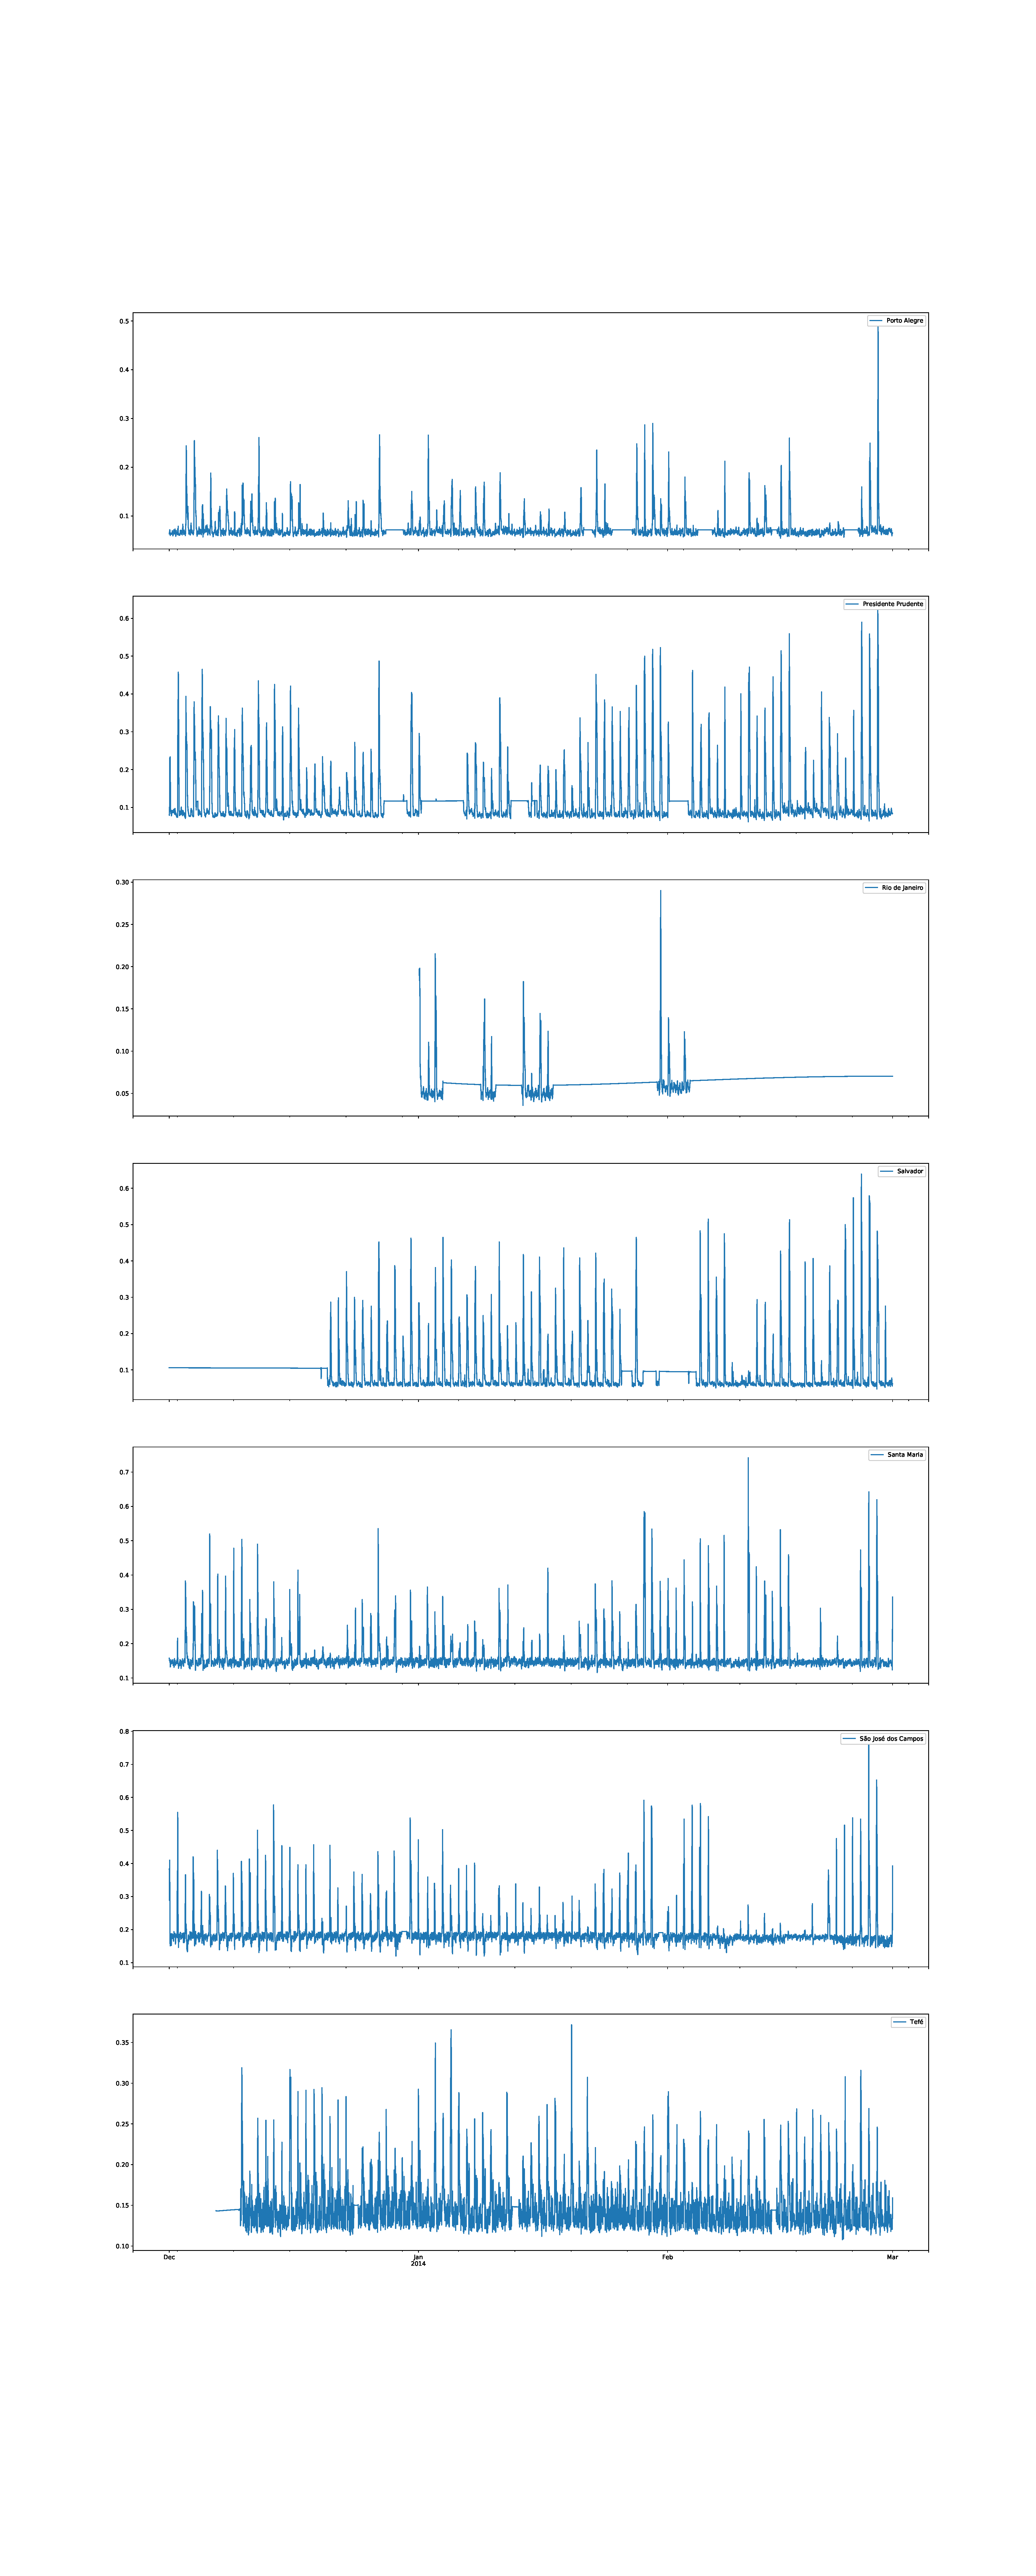
\includegraphics[width=1.5\columnwidth]{./Figuras/s4_stations2.eps}}
\label{fig:s4stations2}
\caption{Amostra do sinal S4 para o terceiro subconjunto de estações.}
\end{figure}

\section{Análises: S4$\times$VTEC em São José dos Campos}

Existem várias formas de se buscar por padrões e correlações em um conjunto de dados, tal como a visualização por meio da plotagem de um gráfico representativo de uma série temporal. Assim, a seção \ref{sec:viss4vtec} forneceu um indicativo da correlação em sua conclusão. Observado tal fato o próximo passo é buscar por um modelo que faça um mapeamento entre VTEC e S4. Este pode ter como conjunto de entrada o valor de VTEC e o de saída o S4, uma vez que ambas as variáveis são contínuas, busca-se realizar uma regressão. 

Poder-se-ia buscar um mapeamento tal que a cada valor de VTEC seja associado a um valor de S4 por estação, entretanto, usando os padrões observados juntamente das referências \cite{}, derivou-se um conjunto adicional de variáveis, que são a derivada temporal primeira e segunda do VTEC, a diferença do VTEC entre São José dos Campos e Pirassununga, a diferença do VTEC entre São José dos Campos e Brasília, assim como as derivadas temporais primeira de ambas as diferenças. 

As derivadas temporais são interessantes, pois os valores de S4 aumentam conforme o valor de VTEC diminui, portanto existe uma variação no tempo que pode ser melhor extraída pela derivada temporal. As bolhas ionosféricas se deformam e se propagam ao longo de um meridiano magnético, as estações de Brasília, Pirassununga e São José dos Campos se encontram aproximadamente sobre o mesmo meridiano magnético, usando ambos os fatos considere que exista uma bolha em Brasília, e não em São José dos Campos, a diferença de VTEC terá um valor positivo, enquanto que se estiverem em ambas as cidades ter-se-á um valor aproximadamente nulo, e com a bolha apenas em São José dos Campos um valor de diferença negativa, isto exibe claramente a propriedade da diferença espacial do VTEC em mapear a localização da bolha. A derivada temporal das diferenças espaciais fornece um indicativo da dinâmica da bolha.

Sumarizando, ficou-se com o seguinte conjunto de variáveis, atributos, mais uma variável alvo S4:

\begin{itemize}
\item {\bf vtec} - conteúdo eletrônico total vertical;
\item {\bf vtec\_dt} - diferença finita de primeira ordem no tempo do VTEC, calculada por $vtec_i-vtec_{i-1}$;
\item {\bf vtec\_dt2} - diferença finita de segunda ordem no tempo do VTEC, calculada por $vtec_{i+1}-2vtec_i+vtec_{i-1}$;
\item {\bf gvtec1} - diferença entre o VTEC de São José dos Campos e Pirassununga;
\item {\bf gvtec1\_dt} - diferença finita de primeira ordem no tempo do gvtec1, calculada por $gvtec1_i-gvtec1_{i-1}$;
\item {\bf gvtec2} - diferença entre o VTEC de São José dos Campos e Brasília;
\item {\bf gvtec2\_dt} - diferença finita de primeira ordem no tempo do gvtec1, calculada por $gvtec2_i-gvtec2_{i-1}$;
\item {\bf S4} - índice de cintilação ionosférico em São José dos Campos;
\end{itemize}

O papel do notebook 06\_analise\_sj2.ipynb é o de construir as variáveis definidas, assim como o de concatenar tais variáveis em uma tabela que possa ser utilizada em algoritmos de aprendizagem de maquina para desenvolvimento de um modelo.

Em posse desse conjunto de variáveis utilizou-se de um método de normalização para restringir o valor destas ao intervalo $[0,1]$ seguindo do treinamento de uma árvore de regressão, uma floresta randômica de regressão e uma máquina de suporte vetorial também de regressão. Esses modelos foram desenvolvidos respectivamente nos notebooks 07\_analise\_sj2\_tree.ipynb, 07\_analise\_sj2\_random\_forest.ipynb e 07\_analise\_sj2\_svm.ipynb. Além disso, para todos os modelos, seguiu-se com uma análise de sensibilidade aos atributos, removendo uma variável de cada vez, gerando então um novo modelo e avaliando as métricas deste.
